\chapter{Architektury her}
V této kapitole si rozebereme architektury, které lze využít pro vývoj her. Pomůže nám to lépe porozumět problémům, které ECS řeší. Začneme objektovým návrhem a prozkoumáme problémy spojené s dědičností při vývoji her. Následně se zaměříme na návrhový vzor Component, který se snaží řešit tuto problematiku, a nahlédneme proč komunikace mezi komponentami může být problematická.

% Iterativni proces
Proto, abychom lépe porozuměli herním architekturám, bude nutné si nejprve přiblížit, jak se tvorba her liší od tvorby jiného typu softwaru. Vývoj her je iterativní proces, při kterém se nejprve navrhnou herní mechaniky. Následně probíhá testování, při kterém se zjistí, jestli jsou příslušné herní mechaniky zábavné. Pokud nejsou, je nutné je upravit a znovu otestovat. Tyto dvě aktivity se opakují, dokud vytvořené mechaniky nejsou dostatečně zábavné. V moment, kdy jsou mechaniky vytvořené a víme o nich, že jsou zábavné, je možné vytvořit další mechaniky a celý proces opakovat. Takto se postupuje, dokud nedojde k vytvoření celé hry.

% Co to implikuje?
Výše zmíněný iterativní proces nám implikuje, že zdrojový kód pro hry se mění velice často. Z toho důvodu je flexibilita velmi důležitou vlastností architektury při vývoji her.

\section{Objektový návrh}
% prirozenym zpusobem vyuzit bezneho objektoveho navrhu programovaciho jazyka, cili udelat nejakou sadu objektu provazanych dedicnosti
Přirozeným přístupem pro tvorbu softwaru je použití objektového návrhu a s jeho pomocí si vytvořit sadu tříd provázaných dědičností. Ovšem jak již bylo naznačeno, v případě tvorby her může být tento přístup problematický.

% Jak se pouziva objektovy návrh ve vyvoji her

Navrhneme si jednoduchou hru, na které si přiblížíme problémy s dědičností, které mohou při vývoji her s objektovým návrhem nastat. Budeme navrhovat jednoduchý tower defense. Začneme třídou \verb|GameObject|, ta nám bude sloužit jako předek pro libovolný objekt ve scéně. Nyní bychom chtěli vytvořit jednotky, vytvoříme tedy třídu \verb|Unit|, která podědí od \verb|GameObject|. Chtěli bychom, aby ve hře byly také speciální jednotky, které umí střílet, například lučištníci. Vytvoříme tedy třídu \verb|Archer|, která dědí od třídy \verb|Unit|. Dále v naší hře budeme potřebovat věže, uděláme tedy třídu \verb|Tower|, dědicí od třídy \verb|GameObject|. Určitě budeme chtít, aby většina našich věží uměla střílet, implementujeme tedy další třídu \verb|ShootingAbleTower|, dědicí od třídy \verb|Tower|. Do této třídy budeme určitě chtít implementovat mechaniku střelby. Ovšem střelbu jsme již určitě implementovali do třídy \verb|Archer|, což nám nyní vytváří duplicitní kód. Celou situaci je možné vidět na obrázku \ref{fig:inheritance}.

\begin{figure}
    \centering
    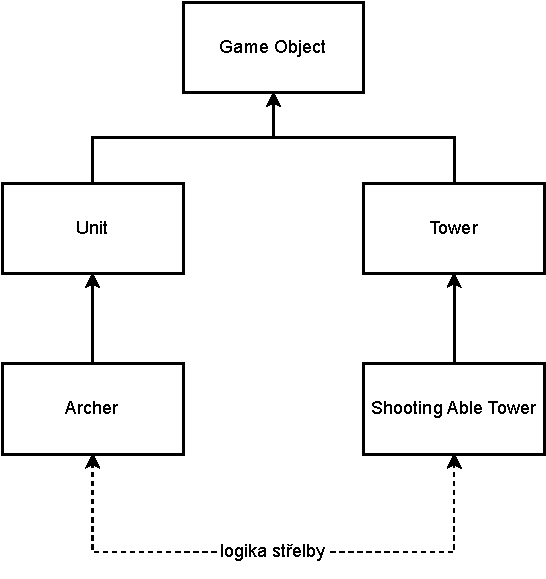
\includegraphics[width=0.6\linewidth]{img/inheritance.pdf}
    \caption{Diagram znázorňující dědičnost tříd ShootingAbleTower a Archer.}
    \label{fig:inheritance}
\end{figure}

Jak tento problém vyřešit? Prvním přístupem je využití \textit{multiple inheritance} \xxx{link} (vícenásobné dědičnosti). Pokud programovací jazyk povoluje \textit{multiple inheritance}, umožňuje to jedné třídě mít více než jednoho předka. Pokud bychom chtěli pomocí \textit{multiple inheritance} vyřešit náš problém, mohli bychom implementovat třídu \verb|ShootingAble|, která dědí od \verb|GameObject|. Do této třídy bychom implementovali mechaniku střelby. Náš \verb|Archer| by poté dědil od \verb|ShootingAble| a od \verb|Unit|. Naše \verb|ShootingAbleTower| by dědila od \verb|ShootingAble| a od \verb|Tower|. Situaci je možné vidět na obrázku \ref{fig:diamong_problem}.

\begin{figure}
    \centering
    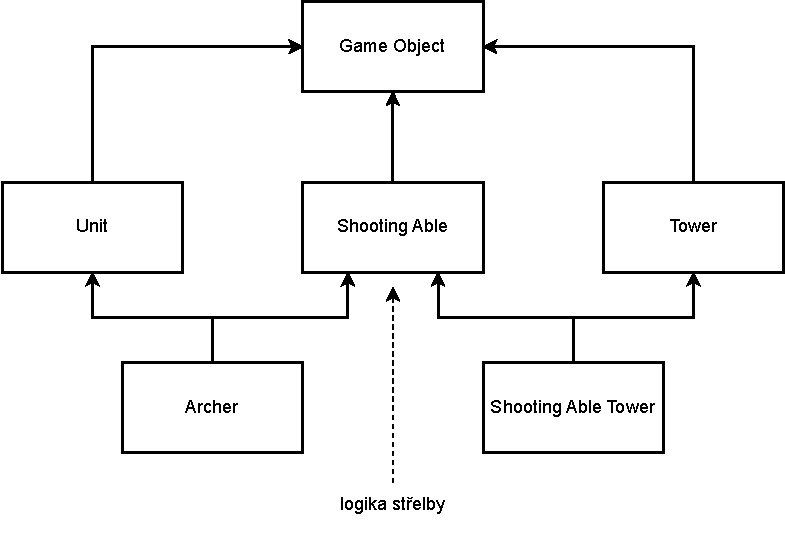
\includegraphics[width=0.6\linewidth]{img/diamond_problem.pdf}
    \caption{Diagram znázorňující dědičnost tříd ShootingAbleTower a Archer při použití multiple inheritance.}
    \label{fig:diamong_problem}
\end{figure}

Tímto řešením by nám ale vznikl takzvaný \textit{diamond problém} \xxx{link}. Jedná se o problém, který může vzniknout při používání \textit{multiple inheritance}. \textit{Diamond problém} nastává tehdy, pokud je potřeba přistoupit ke členům definovaným na společném předkovi. V našem případě se jedná o členy na třídě \verb|GameObject|.

Alternativním přístupem by mohlo být přesunutí společné logiky do společného předka. V našem případě bychom mechaniku střelby implementovali přímo ve třídě \verb|GameObject|.

Ovšem tímto porušíme jeden z principů objektového programování, konkrétně \textit{single responsibility} \xxx{link}. Tento princip nám říká, že každá třída by měla být zodpovědná pouze za jednu věc. Porušení tohoto principu může mít za následek, že se nám ve společném předkovi začne hromadit velké množství logiky. To může vyústit v obrovskou třídu, která řeší všechny možné herní mechaniky. Jedná se o takzvaný \textit{blob object} \xxx{link}. 

Další problém je, že náš návrh je příliš závislý na hierarchii dědičnosti, což omezuje design naší hry. V praxi to znamená, že například není možné za běhu přidat objektu schopnost střílet.

Řešením celé této situace je koncept \textit{composition over inheritance} \xxx{link}. Tento koncept nám říká, že namísto hluboké hierarchie dědičnosti bychom měli preferovat rozdělení objektů do komponent. Je to princip, na kterém je postavený návrhový vzor Component a také ECS.

\section{Návrhový vzor Component}
\label{sec:component}
Component je návrhový vzor, který se často používá pro vývoj her. Používá jej velké množství herních frameworků a enginů, jako je například Unity nebo MonoGame. Jak jsme již zmínili v úvodu, návrhový vzor Component je velice dobře popsán v knize Game Programming Pattern~\cite{nystrom2014game}.
% Unreal, Unity, MonoGame
% odkaz na game programming patterns

% citace na component
Přibližme si co to vlastně je návrhový vzor Component. Máme nějakou entitu (neplést s entitou z ECS, která reprezentuje pouze objekty v herní scéně), například hráče nebo přímo celou hru. Tato entita obsahuje několik domén. Pro hráče to mohou být logiky, které řeší například útok nebo pohyb. Pro hru to mohou být jednotlivé herní mechaniky, jako například spawnování nepřátel nebo čtení vstupu z klávesnice. Abychom izolovali tyto domény, tak kód každé takové domény umístíme do samostatné komponenty. Tato komponenta může být reprezentována například třídou. Entita jako taková je redukována na kontejner těchto komponent. Použitá definice pochází z již zmíněné knihy Game Programming Patterns~\cite{nystrom2014game}.

% \xxx{A single entity spans multiple domains. To keep the domains isolated, the code for each is placed in its own component class. The entity is reduced to a simple container of components.}

% Jeho pouziti se muze lisit
Je vidět, že tento návrhový vzor je definován velice obecně. Jeho implementace a použití se v praxi mohou lišit. Ve skutečnosti je tento návrhový vzor použit i v ECS, konkrétně pro komponenty jednotlivých entit. V této sekci se ale budeme bavit o použití tohoto návrhového vzoru jako architektury pro vývoj her.

% Jak ho pouziva Unity
Nyní si přibližme, jak se návrhový vzor Component používá v herním enginu Unity. V Unity je každý objekt ve scéně reprezentován třídou \verb|GameObject|. Každý takový objekt má interně v sobě kontejner, který obsahuje komponenty, kterými objekt disponuje. Důležitým typem komponenty, který entita může mít, jsou skripty. Pomocí skriptů si uživatel Unity může dodefinovat chování pro jednotlivé herní objekty ve scéně. Každý takovýto skript dědí od abstraktní třídy \verb|MonoBehaviour|. Tyto skripty společně s ostatními komponentami, které na sobě jednotlivé herní objekty mohou mít, jsou typickým příkladem návrhového vzoru Component.

% Jak ho pouziva MonoGame
Na druhou stranu MonoGame, herní framework pro C\#, volí jiný způsob a jako danou entitu z definice zvolil hru samotnou. Jakákoliv herní komponenta dědí od abstraktní třídy \verb|GameComponent|. Hra má interní kolekci, kde uchovává všechny instance herních komponent. MonoGame má také abstraktní třídu \verb|DrawableGameComponent|, která dědí od \verb|GameComponent| a přidává herním komponentám, které od ní dědí, schopnost se vykreslit.

Jak je vidět u Unity i MonoGame, komponenty bývají často reprezentovány jako třídy, které dědí od abstraktního předka. To jim umožňuje provést přetížení některých funkcí, které na sobě předek definuje. Ovšem to má za následek, že implementace návrhového vzoru Component je závislá na volání virtuálních funkcí, které může být výkonnostně neefektivní.

Další výkonnostní problém spočívá v neefektivním používání paměti. Jelikož jsou potřebné virtuální funkce, je nutné jednotlivé komponenty reprezentovat jako pointery (nebo referenční typy). Tím pádem nevyužívají efektivně cache.

Dalším problémem návrhového vzoru Component je komunikace mezi jednotlivými komponentami. Jedním z přístupů, jak komunikaci mezi komponentami vyřešit, je, že si z jedné komponenty vezmeme referenci na jinou komponentu. Tím umožníme, že tyto komponenty mohou spolu komunikovat. Ovšem tím nám vznikne \textit{tight coupling} \xxx{link}. Jedná se o situaci, kde dvě nebo více komponent (ne nutně komponent z návrhového vzoru Component nebo z ECS) je na sobě závislých. To může vyústit například v to, že pokud budeme chtít provést změny v jedné komponentě, bude to vyžadovat provést změny také v jiné komponentě. Problematika komunikace mezi komponentami je Více prozkoumána v již zmiňované knize Game Programming Patterns~\cite{nystrom2014game}.

% Veci jsou vysvetlene ale nevysel z nich zadny vysledek. Bude v kapitole 3?